
\documentclass[12pt,a4paper]{article}
\usepackage[utf8]{inputenc}
\usepackage[english,russian]{babel}
\usepackage{indentfirst}
\usepackage{misccorr}
\usepackage{graphicx}
\usepackage{amsmath}

%\graphicspath{{pictures/}}
\DeclareGraphicsExtensions{.pdf,.png,.jpg, .mps, }


\begin{document}






\begin{titlepage}

 \begin{center}
 Московский Государственный Университет имени М.В.Ломоносова \\
Механико-математический факультет\\
Кафедра теории вероятностей
  \end{center}

 \vspace{3cm}
 
 \begin{center}
   
  {  Курсовая работа за 3 курс:\\
  Об оптимальности основных принципов назначения премий}
   
    \vspace{5cm}
\end{center}     
   
     
   \hspace{170pt}  {Выполнила: Александра Токаева,  309 \\}
       
 \vspace{0.1cm}
  \hspace{170pt} 	  Научный руководитель:  проф. Г.И.Фалин\\

\vspace{4cm}

  \begin{center}
  {Москва\\
  2020}
  \end{center}  
  
\newpage
\tableofcontents
 
 
\end{titlepage}

\section{ От автора}


Задача назначения страховых премий и определения оптимальной цены для различных финансовых инструментов играет важнейшую роль в страховой 
математике, поскольку без правильно назначенной цены на продукт  его нельзя продать и получить прибыль. Цель данной работы -- подробно  и основательно изучить этот раздел современной теории страхования,   дать описание  основных подходов к назначению премий и сделать определенные выводы. Наши рассуждения опираются на статью G.Falin. On the optimal pricing of a heterogeneous portfolio. Astin Bulletin, 2008, 38(1), pp.161-170.  Отметим, что  некоторые рассуждения  и логические переходы в данной статье содержат пропуски или вовсе опущены. Мы полностью восстановим все пропущенные рассуждения и добавим важные, на наш взгляд, детали. К таким мы относим, например, альтернативные решения задач 1 и 2,  использующие  не неравенство Коши-Буняковского-Шварца, а минимизационные  свойства перпендикуляра, опущенного из точки на гиперплоскость, и  геометрические свойства скалярного произведения векторов соответственно.
Однако мы не претендуем на авторство конкретных утверждений и результатов, а также используемых понятий из теории вероятностей и страхования, поэтому вся работа, проделанная лично нами,  отдельно отмечена.  \\
Мы применим простые геометрические принципы, чтобы найти оптимальные значения премий и минимизировать вероятность разорения. Кроме того, мы покажем, что три стандартных подхода  к назначению премий (имеются в виду принципы деления добавочной суммы пропорционально ожидаемому убытку, дисперсии или среднеквадратическому отклонению) являются частными случаями рассматриваемой нами задачи  оптимизации и при этом  минимизируют  взвешенные  ожидаемые квадраты разностей  как между индивидуальными премиями и индивидуальными выплатами,   так и между суммарными премиями для классов однородных рисков и суммарными выплатами по этим классам. \\


 \section{ Постановка задачи }
 
Рассмотрим портфель из $n$ неоднородных независимых страховых рисков. Пусть  $X_{i} $  обозначает размер выплат по  $i$-му риску за рассматриваемый период, 
$S = X_{1} + \dots + X_{n} $ -- суммарные потери, связанные с портфелем. При некоторых естественных предположениях (что портфель достаточно большой, не очень неоднородный и распределение размера выплат не очень ассиметричное) распределение случайной величины $\frac{S-ES}{\sqrt{VarS}}$ может быть приближено стандартным гауссовским распределением.\\

 \begin{figure}[h]
\center{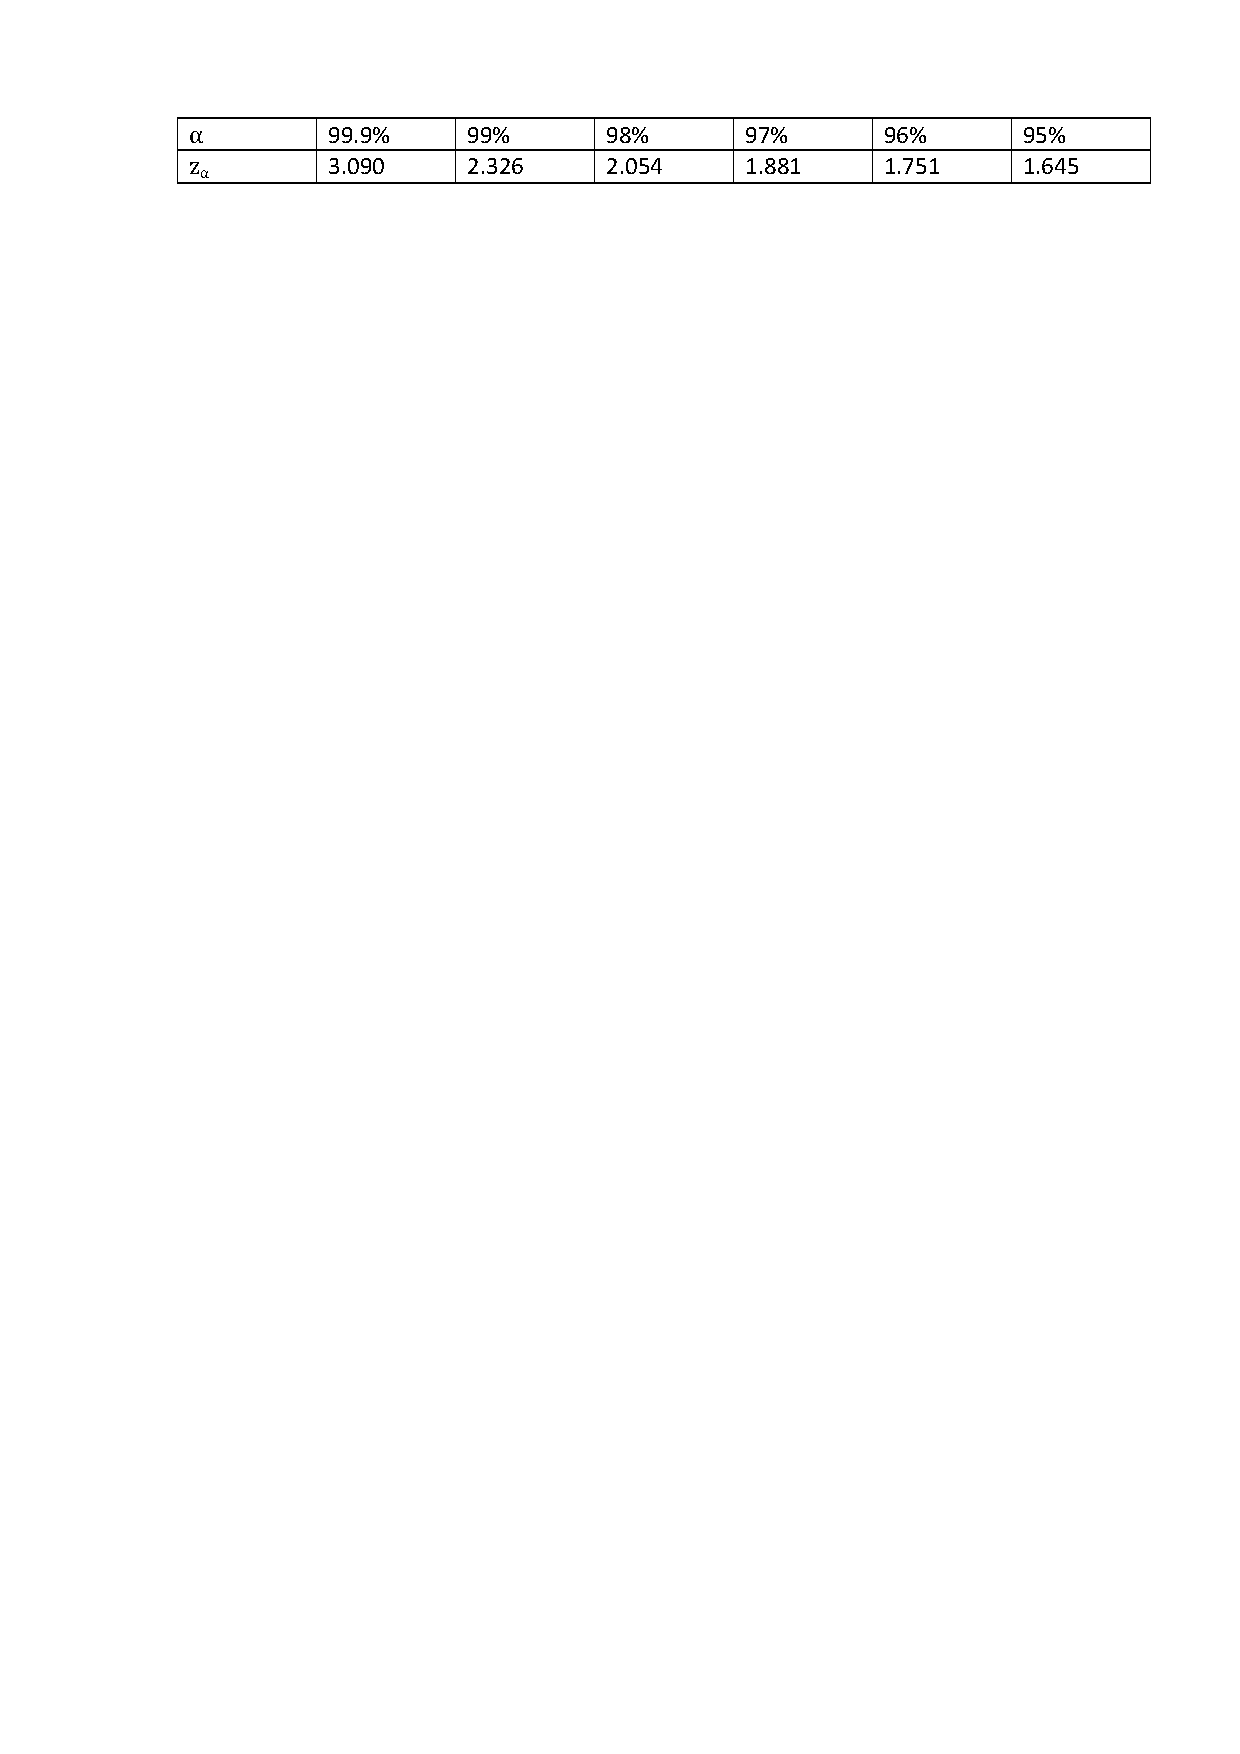
\includegraphics[scale=0.9]{table.pdf}}
\caption{ Квантили стандартного нормального распределения}
\label{fig:image}
\end{figure}

Предположим, что страховщик взимает премию $\pi_i$ по $i-$му  риску и таким образом собирает суммарную премию  $\pi=\sum \limits_{i=1}^{n}\pi_i$.
 Из приблизительной гауссовости  распределения  величины $\frac{S-ES}{\sqrt{VarS}}$ получаем, что для гарантии достаточно маленькой вероятности разорения $R=P(S>\pi)$ (например, $R=5\%$) страховщик должен собрать суммарную премию в размере 
$$ES + \sqrt{VarS}*z_{1-R} \eqno(1) $$ где $z_{\alpha} $
 - квантиль гаусовского распределения уровня $\alpha$.
 
 \begin{figure}[h]
\center{\includegraphics[scale=0.9]{pictures1.mps}}
\caption{ Квантиль уровня $\alpha $}
\label{fig:image}
\end{figure}




Поясним последнее утверждение: 
$$P(S>\pi)=R $$
$$\Leftrightarrow P(\frac{S-ES}{\sqrt{VarS}} > \frac{\pi-ES}{\sqrt{VarS}})=R $$
$$\Leftrightarrow \frac{\pi-ES}{\sqrt{VarS}}=z_{(1-R)}$$
$$ \Leftrightarrow \pi=ES + \sqrt{VarS}*z_{(1-R)}.$$\\

Последнее равенство ничего не говорит о величине индивидуальных премий. Чтобы найти их, необходимо использовать дополнительные принципы, описанные далее. 
Но сначала в качестве иллюстрации мы применим гауссовское приближения для решения следующей задачи. \\

\section{ Пример $1$}
 Предположим, что в компании застраховано $N=3000$ человек с вероятностью смерти в течение года $q=0.3\% = 0.003.$ 
Компания выплачивает сумму $b = 250000$ руб. в случае смерти застрахованного в течение года и не платит ничего, если этот человек доживет до конца года.\\
Определите величину активов, достаточную, чтобы обеспечить вероятность разорения порядка $5\%.$\\

{\bf Решение:} Как обычно, примем размер страховой премии в качестве новой денежной единицы.\\
Прежде всего, мы должны подсчитать среднее значение и дисперсию суммарного ущерба $S.$\\
$$ES = N E \xi = 3000 \cdot 0.003 = 9.$$
$$VarS = N Var \xi = 3000(b^2q - (bq)^2) = 3000 \cdot 0.997 \cdot 0.003 \approx 9.$$
Поэтому 
$$P(S \leq u) = P\left( \frac{S-ES}{\sqrt{VarS}} \leq  \frac{u-ES}{\sqrt{VarS}} \right) 
=  P\left( \frac{S-ES}{\sqrt{VarS}} \leq  \frac{u-9}{3} \right) \approx \Phi\left( \frac{u-9}{3} \right).$$

Если мы хотим, чтобы вероятность разорения была $5\%,$ то величина $\frac{u-9}{3}$ 
должна быть равна $z_{95\%} = 1.645,$ то есть $u=3\cdot 1.645 + 9 \approx 13.935$ от величины страховой суммы, то есть 3483750 руб.


{   \section{ Четыре принципа назначения премий }} 


Сначала мы напомним три стандартных принципа назначения премий, а потом предложим четвертый принцип, в рамках которого 
 мы рассмотрим два подхода к задаче разбиения величины $\pi$ на $n$ индивидуальных премий $\pi_1 \ldots \pi_n.$ \\
 
 {\bf Принцип 1  } Будем делить добавочную сумму $l=  \sqrt{VarS}*z_{(1-R)}$ пропорционально ожидаемому убытку $EX_i,$  то есть $l_i = kEX_i.$\\
 Поскольку $\sum l_i = l = \sqrt{VarS}*z_{(1-R)}$ и $\sum EX_i = ES,$  то  суммируя все $l_i = kEX_i, $ получаем $ \sqrt{VarS}*z_{(1-R)} = kES.$\\
 То есть $k=\frac {\sqrt{VarS}*z_{(1-R)} }{ES}, $ \\
 поэтому  $ \boxed  { \pi_i = EX_i +  \frac {\sqrt{VarS}*z_{(1-R)} }{ES}  EX_i } $\\
 
  {\bf Принцип 2  } Будем делить добавочную сумму $l=  \sqrt{VarS}*z_{(1-R)}$ пропорционально дисперсиям  $VarX_i,$  то есть $l_i = kVarX_i.$\\
 Поскольку $\sum l_i = l = \sqrt{VarS}*z_{(1-R)}$ и $\sum VarX_i = VarS,$  то  суммируя все $l_i = kVarX_i, $ получаем $ \sqrt{VarS}*z_{(1-R)} = kVarS.$\\
 То есть $k=\frac {z_{(1-R)} }{\sqrt{VarS}}, $ \\
 поэтому  $ \boxed  { \pi_i = EX_i +  \frac {\sqrt{VarS}*z_{(1-R)} }{VarS}  VarX_i } $\\
 
  {\bf Принцип 3  } Будем делить добавочную сумму $l=  \sqrt{VarS}*z_{(1-R)}$ пропорционально среднеквадратичным 
  отклонениям  $ \sqrt{VarX_i},$  то есть $l_i = k\sqrt{VarX_i}.$\\
 Поскольку $\sum l_i = l = \sqrt{VarS}*z_{(1-R)}$ и $\sum VarX_i = VarS,$  то  суммируя все $l_i = kVarX_i, $
  получаем $ \sqrt{VarS}*z_{(1-R)} = k\sum\limits_{i=1}^{N} \sqrt{VarX_i}.$\\
 То есть $k=\frac {\sqrt{VarS}*z_{(1-R)} }{\sum\limits_{i=1}^{n} \sqrt{VarX_i}}, $ \\
 поэтому  $ \boxed  { \pi_i = EX_i +  \frac {\sqrt{VarS}*z_{(1-R)}  * \sqrt{VarX_i}}{\sum\limits_{i=1}^{n} \sqrt{VarX_i}} }$



 {\bf Принцип 4  }  К нему ведут два разных подхода:\\
 1) Для заданной вероятности разорения $R=P(S>\pi)$  (то есть для заданного значения $\pi=ES + \sqrt{VarS}*z_{(1-R)}$)  назначить индивидуальные премии так, чтобы минимизировать взвешенную среднюю  квадратичную  разность $D= \sum \limits_{i=1}^{n} \frac {1}{s_i} E(X_i-\pi_i)^2$ между индивидуальными рисками $X_i$ и индивидуальными премиями $\pi_i$ (где $s_i$ -- это некоторые известные положительные числа)\\
 2) Для заданной $D=\sum \limits_{i=1}^{n} \frac {1}{s_i} E(X_i-\pi_i)^2$  минимизировать вероятность разорения $P(S>\pi)$\\
 
Сейчас  мы покажем, что оптимальное решение для обоих подходов   одинаково и имеет вид\\
$ \boxed  {     \pi_i =  EX_i +   \sqrt{VarS}*z_{(1-R)}  \cdot \frac{s_i}{\sum\limits_{j=1}^{n} s_j }  }$\\

В частности, если $s_i = EX_i,$ то мы получаем принцип 1, если $s_i = VarX_i,$ то мы получаем принцип 2,  а если $s_i = \sqrt{VarX_i},$ то мы получаем принцип 3.\\ 

Кроме того, мы покажем, что оптимальные премиии $\pi_i$ минимизируют   взвешенную среднюю  квадратичную  разность  как между индивидуальными премиями и индивидуальными выплатами, так и  между суммарными премиями для классов однородных рисков и суммарными выплатами по этим классам. \\


{\section { Общие результаты о случайных величинах}}
{\subsection{  Задача минимизации величины $D$}}

Пусть $\xi_1, \ldots ,\xi_N$ -- случайные величины с конечными матожиданиями $a_1, \ldots ,a_N$ и дисперсиями $Var\xi_1 ,\ldots ,Var\xi_N$. 

Мы предполагаем, что матожидания и дисперсии известны.\\

Нам бы хотелось заменить случайные величины $\xi_1, \ldots , \xi_N$ на неслучайные числа $A_1, \ldots, A_N$ таким образом, чтобы взвешенная сумма 
$$D \equiv \sum \limits_{i=1}^{N} \omega_i E(\xi_i-A_i)^2 \eqno(2)$$
 была бы минимальна. Здесь $\omega_1, \ldots, \omega_N$ - это известные  положительные числа. \\
 
Используя элементарные свойства случайных величин, мы можем переписать $D$ следующим образом:
$$D= \sum \limits_{i=1}^{N} \omega_i E(\xi_i-A_i)^2 = \sum \limits_{i=1}^{N} \omega_i( Var(\xi_i-A_i) + (E(\xi_i-A_i))^2)$$ = $$ \sum \limits_{i=1}^{N} \omega_i( Var(\xi_i-A_i) + (a_i-A_i)^2)= \sum \limits_{i=1}^{N} \omega_i Var\xi_i + \sum \limits_{i=1}^{N} \omega_i( a_i-A_i)^2 \eqno(3)$$\\

Поскольку $\omega_i$ и $Var\xi_i$ фиксированы, то изначальная задача минимизации превращается в задачу нахождения минимального значения функции
$$f(A_1, \ldots, A_N) = \sum \limits_{i=1}^{N} \omega_i( a_i-A_i)^2 $$

Очевидно, оптимальным значением являются $$A_1^*=a_1, \ldots, A_N^*=a_N$$
и минимальное значение этой функции равно нулю. Соответственно, минимальное значение величины $D$ равно $\sum \limits_{i=1}^{N} \omega_i Var\xi_i $\\

Теперь усложним ситуацию,   наложив  дополнительные ограничения на переменные $A_1, \ldots, A_N, $ и получим следующую задачу оптимизации:\\

{\bf Задача 1 } Найти минимальное значение $D(A_1, \dots , A_N) $ при условии, что $$A_1 + \ldots+  A_N=C, \eqno(4)$$ где C-известная константа.\\

Опять перепишем $D$ в виде $$D= \sum \limits_{i=1}^{N} \omega_i Var\xi_i + \sum \limits_{i=1}^{N} \omega_i( a_i-A_i)^2$$ и заметим, 
что поскольку $\omega_i$ и $Var\xi_i$ фиксированы,  то для решения задачи 1 нам достаточно найти минимальное значение функции 
$$ f(A_1, \ldots, A_N) = \sum \limits_{i=1}^{N} \omega_i( a_i-A_i)^2$$ на множестве тех  наборов чисел $(A_1, \dots,A_n),$ 
которые удовлетворяют условию (4): $A_1 + \ldots+  A_N=C.$\\


Для решения задачи 1 введем новые переменные $x_i=\sqrt \omega_i (A_i-a_i)$, то есть 
$A_i=a_i + \frac{1} {\sqrt {\omega_i}} x_i$. Тогда задача 1 превращается в:\\

{\bf Задача $ \bf 1^{'}$ }Найти минимальное значение функции $$g(x_1, \ldots, x_N)= \sum \limits_{i=1}^{N} x_i^2 \eqno(5)$$ при условии, что 
$$\sum \limits_{i=1}^{N} \frac{1}{\sqrt \omega_i} x_i = C - \sum \limits_{i=1}^{N} a_i. \eqno(6) $$\\

Последовательности $X=(x_1, \ldots, x_N)$ и $Y=\left(  \frac{1}{\sqrt {\omega_1} }, \ldots, \frac{1}{\sqrt {\omega_N}} \right)$ 
можно понимать как $N-$ мерные евклидовы векторы в пространстве $R^N$. Соответственно, левая часть равенства (6) есть скалярное произведение X и Y, а функция $g(x_1, \ldots, x_N)$ есть $||X||^2$, где $$||X||= \sqrt{x_1^2+ \ldots+x_N^2}$$ - это длина вектора  $ X.$\\

Продолжим решать задачу $1^{'}, $ используя  неравенство Коши-Буняковского-Шварца, согласно которому для любых двух векторов $X,Y \in R^N$ верно 
$$|X \cdot Y| \leq ||X|| \cdot ||Y||,$$  причем равенство достигается тогда и только тогда, когда $X$ и $Y$ линейно зависимы (в частности, если вектор $Y$ ненулевой, линейная зависимость означает, что $X$ пропорционален $Y$: $ X=t \cdot Y$ для некоторого $t \in R$)\\

Применяя это неравенство, получаем:
$$g(x_1, \ldots, x_N)=||X||^2 \geq \frac{|X \cdot Y|^2}{||Y||^2} = \frac{(C-\sum\limits_{i=1}^{N} a_i)^2}
{\sum\limits_{i=1}^{N} \frac{1}{\omega_i} }  \eqno(7) $$

Поэтому для  векторов $(x_1, \ldots, x_N)$, удовлетворяющих (7), имеем:
$$ \min g(x_1, \ldots, x_N) \geq \frac{(C-\sum\limits_{i=1}^{N} a_i)^2}{\sum\limits_{i=1}^{N} \frac{1}{\omega_i}} 
\eqno(8) $$

Поскольку вектор $Y=\left(  \frac{1}{\sqrt{\omega_1}}, \ldots, \frac{1}{\sqrt{\omega_N}} \right)$ ненулевой 
(из-за того, что $\omega_1, \ldots, \omega_N$ - это известные  положительные числа),
 то равенство в (8) достигается тогда и только тогда когда существует такое $ t$ что 
$$x_i = \frac{1}{\sqrt{\omega_i}} \cdot t , i=1, \ldots, N  \eqno(9)$$

Подставляя выражение  $X=t Y$ в (7), получаем, что  
$$t^2 \frac{||Y||^4}{||Y||^2} = \frac{(C-\sum\limits_{i=1}^{N} a_i)^2}{\sum\limits_{i=1}^{N} \frac{1}{\omega_i} }, $$ 
то есть 
$$ t = \frac{ C-\sum\limits_{i=1}^{N} a_i} {\sum\limits_{i=1}^{N} \frac{1}{\omega_i}},$$

поэтому 
$$ x_i=\frac{1}{\sqrt{\omega_i}} \cdot t  = \frac{1}{\sqrt{\omega_i}}   \frac{ C-\sum\limits_{i=1}^{N} a_i} {\sum\limits_{i=1}^{N} \frac{1}{\omega_i}},$$

откуда и следует  ответ в задаче $1^{'}:$

$$\min  \sum \limits_{i=1}^{N} x_i^2=  \frac{C-\sum\limits_{j=1}^{N} a_j}{\sum\limits_{j=1}^{N} \frac{1}{\omega_j} }$$

Возвращаясь теперь к исходной задаче 1, получаем ее решение в виде:\\


$$A_i=a_i + \frac{x_i}{\sqrt \omega_i} = a_i + \frac{t}{\omega_i}  = a_i + \frac{1}{\omega_i} \frac{C-\sum\limits_{j=1}^{N} a_j}{\sum\limits_{j=1}^{N} \frac{1}{\omega_j} } \eqno(10)$$

$$ \boxed {D_{min}= \sum \limits_{i=1}^{N} \omega_i Var\xi_i  +  \frac{(C-\sum\limits_{j=1}^{N} a_j)^2}
{\sum\limits_{j=1}^{N} \frac{1}{\omega_j}} } \eqno(11) $$


{\subsection{  Альтернативное решение задачи минимизации величины $D$}}



Дадим альтернативное решение задачи минимизации величины $D$, использующее не неравенство Коши-Буняковского-Шварца, а минимизационные свойства перпендикуляра, опущенного из точки на гиперплоскость:\\



{\bf Задача $ \bf 1^{'}$ }Найти минимальное значение функции $$g(x_1, \ldots, x_N)= \sum \limits_{i=1}^{N} x_i^2 $$ при условии, что 
$$\sum \limits_{i=1}^{N} \frac{1}{\sqrt \omega_i} x_i = C - \sum \limits_{i=1}^{N} a_i .$$\\



Опять будем понимать наборы чисел   $X=(x_1, \ldots, x_N)$ и $Y=\left( \frac{1}{\sqrt {\omega_1} }, \ldots, \frac{1}{\sqrt {\omega_N}} \right)$ как  $N$-мерные евклидовы векторы в пространстве $R^N$. Поэтому наша задача заключается в том, чтобы  минимизировать квадрат длины вектора $X, $ удовлетворяющего условию 
$\sum \limits_{i=1}^{N} \frac{1}{\sqrt \omega_i} x_i = C - \sum \limits_{i=1}^{n} a_i $. Но заметим, что данное условие означает, что вектор $X$ принадлежит гиперплоскости с нормалью $Y= \left( \frac{1}{\sqrt {\omega_1} }, \ldots, \frac{1}{\sqrt {\omega_N}} \right).$ \\

Последнее утверждение требует некоторых пояснений. Как известно, гиперплоскость - это линейная поверхность коразмерности один, то есть линейная оболочка
 $ N-1 $   вектора.  Из линейной алгебры известно, что линейные пространства можно задавать системами линейных уравнений, причем   (см. [2]) если система имеет ранг $ k,$ то задаваемое ей пространство будет иметь размерность $N-k.$    Поэтому в  случае  гиперплоскости (размерности  $N-1$)   в $N$-мерном пространстве  требуется всего одно уравнение. Запишем его в виде $b_1x_1 + \dots + b_N x_N=c$. Согласно общей теории, это уравнение задает плоскость размерности $N-1.$  Но с другой стороны, это левую часть этого уравнения можно  можно переписать в виде  скалярного произведения фиксированного вектора $b= (b_1, \ldots, b_N)$ 
 на вектор  $x$ из этой гиперплоскости. То есть вектор $b$ перпендикулярен всем векторам $x$ из этой гиперплоскости, поэтому  $b$ - вектор нормали к данной гиперплоскости.\\

Данное утверждение, сформулированное как  " в ортонормированной  системе координат главный вектор плоскости является и нормальным ее вектором" доказано в [3]. 

\begin{figure}[h]
\caption{Расстояние от точки до гиперплоскости }\label{pic-jan21-2008-01} \unitlength=1.1mm
\begin{picture}(100,70)
\put(10,0){\vector(0,1){60}} \put(0,10){\vector(1,0){90}}
\put(4,6){\vector(3,2){60}}
\put(92,10){$x_1$}\put(10,62){$x_3$}\put(67,45){$x_2$}\put(10,10){\circle*{1}}
\put(11,6){$O$} \qbezier(10,50)(10,50)(80,10)
\qbezier(10,50)(10,50)(55,40)\qbezier(55,40)(55,40)(80,10)
\put(10,10){\line(2,3){21}}\put(31,41.5){\circle*{1}}\put(32,38){$(x_1^*,x_2^*,x_3^*)$}
\put(10,10){\line(3,1){50}}\put(60,26.6){\circle*{1}}\put(52,28){$(x_1,x_2,x_3)$}
\put(34,15){расстояние=$g(x_1,x_2,x_3)$}
\put(70,25){гиперплоскость $\sum\limits_{i=1}^{N}\frac{1}{\sqrt{w_i}}x_i=C - \sum \limits_{i=1}^{N} a_i$}
\end{picture}
\end{figure}



Из курса линейной алгебры известно, что минимизирует расстояние от точки до гиперплоскости - перпендикуляр, опущенный из этой точки на гиперплоскость (это непосредственно следует из многомерной  теоремы Пифагора).\\
Но  выше мы уже пояснили, что нормаль к  нашей гиперплоскости - это вектор $Y, $ поэтому искомый вектор $X$ будет пропорционален $Y:$ \\
 
 
$X=tY,$ то есть $(x_1, \dots, x_n) = t \left( \frac{1}{\sqrt {\omega_1} }, \ldots, \frac{1}{\sqrt {\omega_N}} \right)$\\

Подставим выражение для $X$ в условие  $$(X,Y) = C- \sum \limits_{i=1}^{N} a_i $$\\

Получим $$t||Y||^2 = C -  \sum \limits_{i=1}^{N} a_i $$\\

Откуда следует, что

$$ t =   \frac{ C-\sum\limits_{i=1}^{N} a_i} { ||Y||^2} = \frac{ C-\sum\limits_{i=1}^{N} a_i} {\sum\limits_{i=1}^{N} \frac{1}{\omega_i}}$$

Значит, минимальное значение в задаче $1^{'} $ имеет вид

$$\min  ||X||^2 =  t^2 ||Y||^2 = t(t||Y||^2) = t(C - \sum \limits_{i=1}^{N} a_i ) =  \frac{ (C-\sum\limits_{i=1}^{N} a_i )^2} {\sum\limits_{i=1}^{N} \frac{1}{\omega_i}}$$


Возвращаясь теперь к исходной задаче 1 минимизации величины $D,$ получаем ответ:

$$\boxed{ D_{min}= \sum \limits_{i=1}^{N} \omega_i Var\xi_i  +  \frac{(C-\sum\limits_{j=1}^{N} a_j)^2}
{\sum\limits_{j=1}^{N} \frac{1}{\omega_j}}  }$$





{\subsection { Задача максимизации суммы  $A_1 + \ldots + A_N$ }}
Теперь  изучим двойственную  задачу оптимизации:\\

{\bf Задача 2} Найти максимум суммы $A_1 + \ldots + A_N,$ если  задано 
$$D= \sum \limits_{i=1}^{N} \omega_i E( \xi_i-A_i)^2 \eqno(12)$$



Как и раньше, перепишем $D$ в виде
 $$ D=  \sum \limits_{i=1}^{N} \omega_i E( \xi_i-A_i)^2  = \sum \limits_{i=1}^{N} \omega_i Var\xi_i + \sum \limits_{i=1}^{N} \omega_i( a_i-A_i)^2, $$
 причем отметим такой факт: 
 из этого представления следует, что константа $D$ должна быть больше или равна, чем $\sum \limits_{i=1}^{N} \omega_i Var\xi_i$\\
 
 Поэтому так введенная константа $D'$ будет неотрицательная:
 $$D^{'} = D - \sum \limits_{i=1}^{N} \omega_i Var\xi_i \geq 0 $$

 

После введения величины $D'$ ограничение (12) превращается в 
 $$ D^{'} = \sum \limits_{i=1}^{N} \omega_i( a_i-A_i)^2 $$ 

Вводя $x_i=\sqrt \omega_i (A_i-a_i), A_i=a_i + \frac{1} {\sqrt {\omega_i}} x_i $ мы сводим задачу 2 к следующему виду:\\


{\bf Задача $ \bf 2^{'}$} Найти максимум суммы $\sum \limits_{i=1}^{N} \frac{1}{\sqrt \omega_i} x_i,$ если  задана
сумма $$D^{'} = \sum \limits_{i=1}^{N} x_i^2 \eqno(13)$$

Для решения этой задачи, опять применяем неравенство Коши-Буняковского-Шварца:\\
$$\sum \limits_{i=1}^{N} \frac{1}{\sqrt \omega_i} x_i = X \cdot Y \leq ||X|| \cdot ||Y|| = \sqrt{D^{'}} \sqrt{\sum\limits_{i=1}^{N} \frac{1}{\omega_i}} \eqno(14)$$

Причем равенство в (14) достигается тогда и только тогда, когда существует $ t$ такое что 
$$x_i = \frac{1}{\sqrt{\omega_i}} \cdot t , i=1, \ldots, N  \eqno(15)$$

Подставляя выражение $X=t Y$ в (14), получаем единственное решение 
$$ t = \sqrt{ \frac{D^{'}}{\sum\limits_{i=1}^{N} \frac{1}{\omega_i}}}$$

Тогда 
$$x_i = \frac{t}{\sqrt{\omega_i}}  = \frac{1}{\sqrt{\omega_i}} \sqrt{ \frac{D^{'}}{\sum\limits_{i=1}^{N} \frac{1}{\omega_i}}}$$

Поэтому  искомый максимум в задаче $2^{'}$ равен $\sqrt{D^{'}} \sqrt{\sum\limits_{i=1}^{N} \frac{1}{\omega_i}}.$


Тогда возвращаясь к исходной задаче 2:
$$A_i = a_i + \frac{x_i}{\sqrt{\omega_i}}  = a_i +  \frac{1}{\omega_i} \sqrt{ \frac{D^{'}}{\sum\limits_{i=1}^{N} \frac{1}{\omega_i}}} \eqno(16)$$

Поэтому максимум суммы $A_1 + \ldots + A_N$  равен 
$$ \sum\limits_{i=1}^{N} a_i + \sqrt{ \sum \limits_{i=1}^{N} \omega_i( a_i-A_i)^2  } \sqrt{\sum\limits_{i=1}^{N} \frac{1}{\omega_i}}$$

{\subsection { Альтернативное решение задачи максимизации суммы  $A_1 + \ldots + A_N$ }}
Дадим альтернативное решение задачи $2^{'},$ использующее не неравенство Коши-Буняковского-Шварца, а геометрические свойства скалярного произведения векторов.

{\bf Задача $ \bf 2^{'}$} Найти максимум суммы $\sum \limits_{i=1}^{N} \frac{1}{\sqrt \omega_i} x_i,$ если  задана
сумма $$D^{'} = \sum \limits_{i=1}^{N} x_i^2 $$

Заметим, что нам нужно максимизировать скалярное произведение векторов $X$ и $Y$, причем длины этих векторов заданы, а изменять мы можем только угол  $\beta$ между ними. Но по свойству скалярного произведения двух векторов оно равняется 
$$||X|| \cdot ||Y|| \cdot \cos \beta$$
Тогда поскольку длины обоих векторов заданы, а косинус по модулю не превосходит единицы, то для максимизации этого скалярного произведения достаточно сделать косинус по модулю равным единице, то есть векторы $X$ и $Y$ должны быть коллинеарны. Получаем, что $X=tY,$  и дальше рассуждаем как было описано в (15) и (16).\\


{\section{ Приложение   полученных результатов к модели индивидуального риска}}

 Рассмотрим модель индивидуального риска:\\
$$S= X_1 + \ldots + X_n,$$ где $S$ - общие потери по портфелю, $n$ -  общее число рисков в портфеле, случайная величина $X_i$ обозначает потери по $i-$му риску за рассматриваемый период, 


Мы предполагаем, что случайные величины $X_1, \ldots, X_n$ независимы и имеют конечные матожидания $\mu_1, \ldots, \mu_n$ и дисперсии $\sigma_1^2, \ldots, \sigma_n^2$ соответственно. Тогда случайная величина $S$ имеет конечное матожидание $\mu = \mu_1+ \ldots + \mu_n$ и дисперсию $\sigma^2 = \sigma_1^2+ \ldots + \sigma_n^2.$  Мы также предполагаем, что для достаточно больших $ n$  функция распределения центрированной и нормированной величины полных потерь $\frac {S-\mu}{\sigma}$ может быть приближена функцией распределения стандартной гауссовской величины 
$\Phi(x) =   \frac{1}{\sqrt{2 \pi}} \int \limits_{-\infty}^{x }e^{-\frac{t^2}{2}} dt$, то есть:

$$P \left( \frac{S-\mu}{\sigma} < x \right)  \approx \Phi(x)$$


Предположим, что страховщик взимает премию $\pi_i$ по $i$-му риску, то есть всего собирает сумму $\pi=\sum \limits_{i=1}^{n}\pi_i.$ Тогда вероятность разорения
 дается формулой $ R=P(S>\pi).$\\
Используя гаусовость  $\frac{S-\mu}{\sigma}$, получаем, что:
$$R=P\left( \frac{S-\mu}{\sigma} > \frac{\pi-\mu}{\sigma} \right)  \approx 1 - \Phi \left(  \frac{\pi-\mu}{\sigma} \right). \eqno(17)$$

Предположим, что страховщик готов принять достаточно маленький риск разорения $R$ (например, $R=1\%$). Тогда равенство (17) дает следующую (приближенную) формулу для суммарной премии:

$$\pi = \mu  + \sigma \cdot z_{(1-R)}  \eqno(18),$$ где $z_{\alpha} $
 - квантиль гаусовского распределения уровня $\alpha$, то есть $\Phi(z_{\alpha}) = \alpha$.\\

Равенство (18) ничего не говорит про величины индивидуальных премий $\pi_i.$ Чтобы найти их, нам придется применить дополнительные принципы.

{\subsection { Минимизация  ожидаемой разности между индивидуальными рисками и индивидуальными  премиями при заданной вероятности разорения }}

{\bf Задача 3} Рассмотрим взвешенную среднюю  квадратичную  разность 
$$ D= \sum \limits_{i=1}^{n} \frac{1}{s_i} E( X_i-\pi_i)^2$$
между индивидуальными рисками $X_1, \ldots, X_n$ и индивидуальными премиями $\pi_1, \ldots, \pi_n$ (где $s_1,   
\ldots, s_n$ - это некие известные положительные числа) и найдем минимум D:

$$ D \equiv D(\pi_1, \ldots, \pi_n) \rightarrow min. \eqno(19)$$

Применяя формулу (10) для $N=n, \xi_i=X_i, a_i = \mu_i, A_i=\pi_i, \omega_i=\frac{1}{s_i}, C= \mu + \sigma \cdot z_{(1-R)}$ мы можем утверждать, что минимизационная задача 3  с ограничением (18) имеет единственное решение 

$$  \boxed {\pi_i^* = \mu_i +  \frac{s_i}{\sum\limits_{j=1}^{n} s_j } \cdot \sigma \cdot z_{(1-R)}. } \eqno(20)$$


Пусть теперь портфель неоднородный, но  его можно разбить на $k$ классов однородных рисков с одинаковыми статистическими характеристиками потерь (обычно риски из одного класса принадлежат одному и тому же сектору бизнеса). Пусть $i-$й класс состоит из $n_i$ рисков с одинаковым средним $\mu_i$
и одинаковыми дисперсиями $\sigma_i^2.$ Тогда  величина суммарных  потерь $S_i$  в $i-$м классе  имеет среднее значение $ES_i= n_i \mu_i$ и дисперсию $ Var S_i = n_i \sigma_i^2.$ 
Суммарные потери по всему портфелю есть 
$S= S_1 + \ldots + S_k$, причем $\mu \equiv ES= \sum\limits_{i=1}^{k} n_i \mu_i $ , 
$\sigma^2 \equiv VarS= \sum\limits_{i=1}^{k} n_i \sigma_i^2 $


Из-за  однородности рисков внутри отдельного класса $i$, страховщик должен взимать со всех рисков в этом классе одну и ту же премию $\pi_i.$ Тогда общая премия за все риски в портфеле равна $\pi = \sum\limits_{i=1}^{k} n_i \pi_i.$\\

{\bf Задача 4} Рассмотрим взвешенную среднюю  квадратичную  разность
$$  D= \sum \limits_{i=1}^{k} \frac{1}{r_i} E( S_i-n_i \pi_i)^2$$ между суммарными потерями по разным классам $S_1, \ldots, S_k$ и суммарными премиями $n_1 \pi_1, \ldots, n_k \pi_k$ от этих классов (где $r_1, \ldots, r_k$ - это некоторые известные положительные числа) и минимизируем $D$:

$$D = D \equiv D(\pi_1, \ldots, \pi_k) \rightarrow min. \eqno(21)$$


Для того, чтобы получить предписанную вероятность разорения, нужно, чтобы  выполнялось (18): $\pi = \mu  + \sigma \cdot z_{(1-R)} .$\\

Применяя формулу (10) для $N=k, \xi_i=S_i, a_i = n_i \mu_i, A_i=n_i \pi_i, \omega_i=\frac{1}{r_i}, C= \mu + \sigma \cdot z_{(1-R)}$ мы можем утверждать, что минимизационная задача (19) с ограничением (18) имеет единственное решение 

$$ n_i \pi_i^* = n_i \mu_i +  \frac{r_i}{\sum\limits_{j=1}^{k} r_j } \cdot \sigma \cdot z_{(1-R)}$$
$$\Leftrightarrow   \boxed {\pi_i^* = \mu_i +  \frac{r_i}{n_i \sum\limits_{j=1}^{k} r_j } \cdot \sigma \cdot z_{(1-R)}.} \eqno(22)$$

Теперь вернемся к минимизационной задаче (19) c ограничением (18) и положим для всех рисков из $i-$го класса одинаковое значение параметра $s_i$ равным $\frac {r_i}{n_i}.$ Тогда  из (20) видно, что оптимальное решение для минимизационной задачи 4 совпадает с оптимальным решением минимизационной задачи (21). Таким образом, одни и те же значения премий минимизируют взвешенную среднюю  квадратичную  разность  как между индивидуальными премиями и индивидуальными потерями, так и между суммарными премиями для классов однородных рисков и суммарными потерями для этих классов (но с разными весами).


{\subsection {  Минимизация вероятности разорения при заданной взвешенной средней  квадратичной  разности между индивидуальными рисками и индивидуальными  премиями }}


{\bf Задача 5} Для модели индивидуального риска $$S= X_1 + \ldots + X_n$$ минимизировать вероятность разорения $R=P(S > \pi)$ при заданной величине $$D = \sum\limits_{i=1}^{n} \frac{1}{s_i} E(X_i - \pi_i)^2$$

Поскольку $P(S > \pi)$ уменьшается при увеличивающемся $\pi$, то задача состоит в нахождении максимального значения суммарной премии $\pi= \pi_1+ \ldots + \pi_n.$\\

Применяя формулу (10) для $N=n,  \xi_i = X_i, a_i= \mu_i, A_i= \pi_i , \omega_i= \frac{1}{s_i},$  мы можем утверждать, что минимизационная задача 5   имеет единственное решение 

$$ \boxed {\pi_i^* = \mu_i + s_i  \sqrt{ \frac{D - \sum\limits_{i=1}^{n} \frac{1}{s_i} \sigma_i^2 }{\sum\limits_{i=1}^{n} s_i}}  }\eqno(23)$$


Теперь опять предположим, что портфель может быть разделен на $k$ классов однородных рисков с одинаковыми статистическими свойствами потерь. 
Пусть $ i-$й класс состоит из $n_i$ рисков с одинаковым средним $\mu_i$ и одинаковыми дисперсиями $\sigma_i^2.$ 
Тогда  величина суммарных  потерь $S_i$  в $i-$м классе  имеет среднее значение $ES_i= n_i \mu_i$ и дисперсию $ Var S_i = n_i \sigma_i^2.$ 
Суммарные потери по  всему портфелю есть 
$S= S_1 + \ldots + S_k$, причем $\mu \equiv ES= \sum\limits_{i=1}^{k} n_i \mu_i $ , 
$\sigma^2 \equiv VarS= \sum\limits_{i=1}^{k} n_i \sigma_i^2 $\\
 
Из-за однородности рисков внутри отдельного класса $ i,$ страховщик должен взимать со всех рисков в этом классе одну и ту же премию $\pi_i.$ 
Тогда общая премия за все риски в портфеле равна $\pi = \sum\limits_{i=1}^{k} n_i \pi_i.$\\

Рассмотрим оптимизационную задачу:

{\bf Задача 6} Минимизировать вероятность разорения $R=P(S>\pi)$ при заданной величине 
$$D = \sum\limits_{i=1}^{k} \frac{1}{r_i} E(S_i - n_i \pi_i)^2$$

Поскольку $P(S > \pi)$ уменьшается при увеличивающемся $\pi$, то задача состоит в нахождении максимального значения суммарной премии $\pi= n_1 \pi_1+ \ldots + n_k \pi_k.$\\

Применяя формулу (10) для $N=k, \xi_i=S_i,  a_i= n_i \mu_i, A_i= n_i \pi_i , \omega_i= \frac{1}{r_i},$  мы можем утверждать, что минимизационная задача 6  имеет единственное решение 

$$ \boxed {\pi_i^* = \mu_i + \frac{r_i}{n_i}  \sqrt{ \frac{D - \sum\limits_{i=1}^{k} \frac{1}{r_i} n_i \sigma_i^2 }{\sum\limits_{i=1}^{k} r_i}}  } \eqno(24)$$

Сравнивая формулы (23) и (24), опять видим, что  одни и те же значения премий минимизируют взвешенную среднюю  квадратичную  разность  как между индивидуальными премиями и индивидуальными потерями, так и между суммарными премиями для классов однородных рисков и суммарными потерями для этих классов (но с разными весами).

В заключение приведем пример, иллюстрирующий все три принципа, а также разбиение на классы однородных рисков.\\

\section{ Пример $2$}
 Предположим, что страховая компания заключила $N=10000$ договоров страхования жизни сроком на один год на следующих условиях:
в случае смерти застрахованного в течение года от несчастного случая компания выплачивает выгодоприобретателю 1000000 руб., а в случае смерти в течение года от естественных причин компания выплачивает выгодоприобретателю 250000 руб. Компания не платит ничего, если застрахованный не умрет в течение года. Вероятность смерти от несчастного случая одна и та же для всех застрахованных и равна 0.0005. Вероятность смерти от естественных причин зависит от возраста. В первом приближении можно разбить $N$ застрахованных на две возрастные группы, содержащие $N_1 = 4000$ и $N_2=6000$ человек с вероятностью смерти в течение года $q_1=0.004 $ и $q_2=0.002$ соответственно.\\
Подсчитайте величину премии, гарантирующую вероятность выполнения компанией своих обязательств, равную $95\%.$\\

{\bf Решение:} Примем сумму $250000$ руб. в качестве условной денежной единицы. Тогда для первой группы договоров индивидуальный убыток принимает три значения: 0, 1 и 4 с вероятностями 0.9955, 0.004 и 0.0005 соответственно. Среднее значение и дисперсия величины индивидуального убытка есть
$$m_1 = 1\cdot 0.004 + 4\cdot 0.0005 = 0.006$$
$$\sigma_1^2 = 1^2 \cdot 0.004 + 4^2 \cdot 0.0005 - m_1^2 \approx 0.012.$$

Для второй группы договоров индивидуальный убыток принимает те же три значения 0, 1 и 4, но с другими вероятностями: 0.9975, 0.002 и 0.0005.  В этой группе среднее значение и дисперсия индивидуального убытка есть
$$m_2 = 1\cdot 0.002 + 4\cdot 0.0005 = 0.004$$
$$\sigma_2^2 = 1^2\cdot 0.002 + 4^2\cdot 0.0005 - m_2^2 \approx 0.01.$$

Среднее значение и дисперсия суммарного убытка равны:
$$ES = N_1 \cdot m_1 + N_2 \cdot m_2 = 4000 \cdot 0.006 + 6000 \cdot 0.004 = 48$$
$$VarS = N_1\cdot \sigma_1^2 + N_2\cdot \sigma_2^2 \approx 4000\cdot 0.012 + 6000\cdot 0.01 = 108$$

Для того, чтобы гарантировать $95\%$ вероятность выполнения своих обязательств, резервный фонд компании должен быть $ES+l = 48+l,$ 
где добавочная сумма $l$  равна
$$l = z_{95\%} \cdot \sqrt{VarS} \approx 1.645 \cdot \sqrt{108} \approx 17.095.$$

Рассмотрим теперь вопрос о назначении индивидуальных премий.\\
1)Если добавочная сумма $l$ делится пропорционально матожиданиям, то относительная страховая надбавка $\theta$ 
одна и та же для всех договоров и равна $$\theta = \frac{l}{ES} \approx 35.6\%$$

Поэтому для договоров из первой группы премия равна
$$\pi_1 = m_1(1+\theta) \approx 0.00814 = \bf 2034 p.$$

Для договоров из второй группы премия равна
$$p_2=m_2(1+\theta) \approx 0.00542 = \bf 1356 p.$$

2)Если добавочная сумма $l$ делится пропорционально дисперсиям, то коэффициент пропорциональности $k$ есть
$$k = \frac{l}{VarS} \approx 15.8\%$$

Поэтому для договоров из первой группы страховая надбавка равна 
$$l_1 = k\cdot \sigma_1^2 \approx 0.001899,$$
так что премия есть
$$\pi_1 = m_1 + l_1 \approx 0.007899 = \bf1975p,$$
а относительная страховая надбавка равна
$$\theta_1 = \frac{l_1}{m_1}  \approx 31.7\%.$$

Для договоров из второй группы страховая надбавка равна 
$$l_2 = k\cdot \sigma_2^2 \approx  0.001583,$$
так что премия есть
$$\pi_2 = m_2 + l_2 \approx 0.005583 = \bf 1396p,$$
а относительная страховая надбавка равна
$$\theta_2 = \frac{l_2}{m_2}  \approx 39.6\%.$$

3) Если добавочная сумма $l$ делится пропорционально среднеквадратическим отклонениям (они равны $\sigma_1 \approx 0.1095$ для договоров первой группы и $\sigma_2 = 0.1$ для договоров второй группы), то коэффициент пропорциональности $k$ есть
$$k = \frac{l}{N_1\sigma_1 + N_2\sigma_2} \approx 0.0165,$$

Поэтому для договоров из первой группы страховая надбавка равна 
$$l_1=k\cdot \sigma_1 \approx 0.001804,$$
так что премия есть 
$$\pi_1 = m_1 + l_1 \approx 0.007804 = \bf 1951p,$$
а относительная страховая надбавка 
$$\theta_1 = \frac{l_1}{m_1}  \approx 30\%.$$

Для договоров из второй группы страховая надбавка равна 
$$l_2=k\cdot \sigma_2 \approx 0.001647,$$
так что премия есть 
$$\pi_2 = m_2 + l_2 \approx 0.005647 = \bf 1412p,$$
а относительная страховая надбавка 
$$\theta_2 = \frac{l_2}{m_2}  \approx 41\%.$$

Итак, изменение принципа назначения индивидуальных премий приводит к уменьшению относительной страховой надбавки для договоров первой группы: 
$\theta_1 = 35.6\%,31.7\%,30\%.$\\
Соответственно для договоров второй группы относительная защитная надбавка увеличивается: 
$\theta_2 = 35.6\%,39.6\%,41\%.$ Это связано с тем, что коэффициент рассеяния суммарного ущерба есть
$$ \frac{VarS}{ES} -1 =1.25,$$
в то время как для договоров первой (второй) группы он равен 
$$\frac{\sigma_1^2}{m_1} - 1= 1$$ и  
$$\frac{\sigma_2^2}{m_2} - 1= 1.5$$ соответственно.\\
Коэффициент вариации величины индивидуального убытка для договоров первой группы есть 
$$c_1 = \frac{\sigma_1}{m_1} \approx 18.26,$$
а для договоров второй группы он равен
$$c_2 = \frac{\sigma_2}{m_2} =25.$$

Средний коэффициент вариации, усредненный по всему портфелю с весами $\frac{E\xi_i}{ES} $ есть
$$c = c_1 \cdot \frac{N_1m_1}{ES} + c_2 \cdot \frac{N_2m_2}{ES} $$
$$=c_1 \cdot \frac{24}{48} + c_2 \cdot \frac{24}{48} = \frac{c_1 + c_2}{2} \approx 21.63.$$

Итак, хотя дисперсия величины индивидуального убытка для договоров второй группы меньше, чем для договоров первой группы 
( $\sigma_2 = 0.1 < \sigma_1 \approx 0.1095 $), но флуктуации индивидуальных убытков для договоров второй группы (измеренные как коэффициентом рассеяния, так и коэффициентом вариации) превышают средние флуктуации по портфелю. Поэтому было бы оправдано выбрать для назначения премий принцип 2 или 3.



\section{ Выводы и замечания}
Таким образом, мы изучили четыре основных  принципа назначения премий: принципы деления добавочной суммы пропорционально матожиданиям, дисперсиям и среднеквадратическим отклонениям индивидуальных рисков, а также более общий способ: способ минимизации  взвешенной средней  квадратичной  разности  $D$ между индивидуальными премиями и индивидуальными потерями. При этом мы изучили два подхода к получению четвертого способа: \\
1)Для заданной вероятности разорения  $P(S>\pi)$ минимизировать взвешенную среднюю  квадратичную  разность  $D=\sum \limits_{i=1}^{n} \frac {1}{s_i} E(X_i-\pi_i)^2$ \\
 2) Для заданной $D=\sum \limits_{i=1}^{n} \frac {1}{s_i} E(X_i-\pi_i)^2$  минимизировать вероятность разорения $P(S>\pi)$\\
 Кроме того, мы увидели, что оба подхода имеют одно и то же решение, которое к тому же минимизируют взвешенную среднюю  квадратичную  разность  как между индивидуальными премиями и индивидуальными потерями, так и между суммарными премиями для классов однородных рисков и суммарными потерями для этих классов (но с разными весами).\\
Однако необходимо подчеркнуть, что мы использовали лишь простейшую модель для расчета защитной надбавки ( через приближение  центрированной и нормированной величины суммарных  потерь нормальным распределением). Вопрос о том, что делать, когда  нельзя применять эту модель,  заслуживает  отдельного обсуждения, выходящего за рамки данной работы.




\section{ Литература}

$\bullet$ [1] G.Falin. On the optimal pricing of a heterogeneous portfolio. Astin Bulletin, 2008, 38(1), pp.161-170. \\
$\bullet$ [2] Шурыгин В.B, Аналитическая геометрия, часть 3, стр. 4\\
$\bullet$ [3] A.E.Умнов,  Аналитическая геометрия и линейная алгебра, Москва, МФТИ, 2011, стр. 99\\








\end{document}
